\documentclass[a4paper,11pt]{article}

\usepackage[T1]{fontenc}
\usepackage[utf8]{inputenc}
\usepackage[english,polish]{babel}
\usepackage{lmodern}
\usepackage{graphicx}
\usepackage{fancyhdr}
\usepackage{float}
\usepackage{array}

\usepackage{mathtools}


\setlength{\textheight}{23.5cm}
\setlength{\textwidth}{15.92cm}
\setlength{\footskip}{10mm}
\setlength{\oddsidemargin}{0mm}
\setlength{\evensidemargin}{0mm}
\setlength{\topmargin}{0mm}
\setlength{\headsep}{15mm}
\setlength{\parindent}{0cm}
\setlength{\parskip}{2.5mm}
\title{Projekt filtru}
\author{Justyna Ilczuk, Jacek Rosiński}
\begin{document}
\maketitle

Dane: 
\( N = 3 \), \( f_g = 600 Hz \), \( k = 2.5 \) \\
Rodzaj filtru:
filtr Butterswortha

Obliczenia zostały wykonane za pomocą programu maxima.  \\
Dla współczynników równych: \\
\(a_1 = 1 \),
\(b_1 = 1 \),
\(a_2 = 1 \),
\(b_2 = 0 \)

Dalej dołączamy stronę z obliczeniami.

Wykresy zostały wykonane za pomocą programu gnumeric, a schemat za pomocą programu KolourPaint.

\begin{figure}
\begin{flushleft}
\includegraphics[scale=0.4]{schemat}
\caption{Schemat filtru}
\end{flushleft}
\end{figure}

\begin{figure}
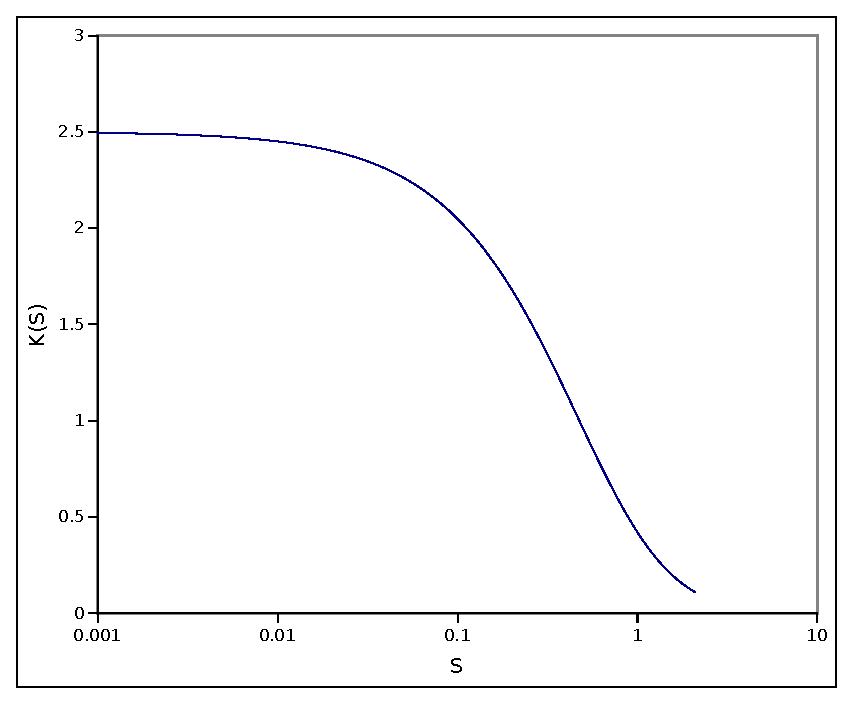
\includegraphics[scale=1]{charakterystyka_liniowa}
\caption{Charakterystyka liniowa}
\end{figure}

\begin{figure}
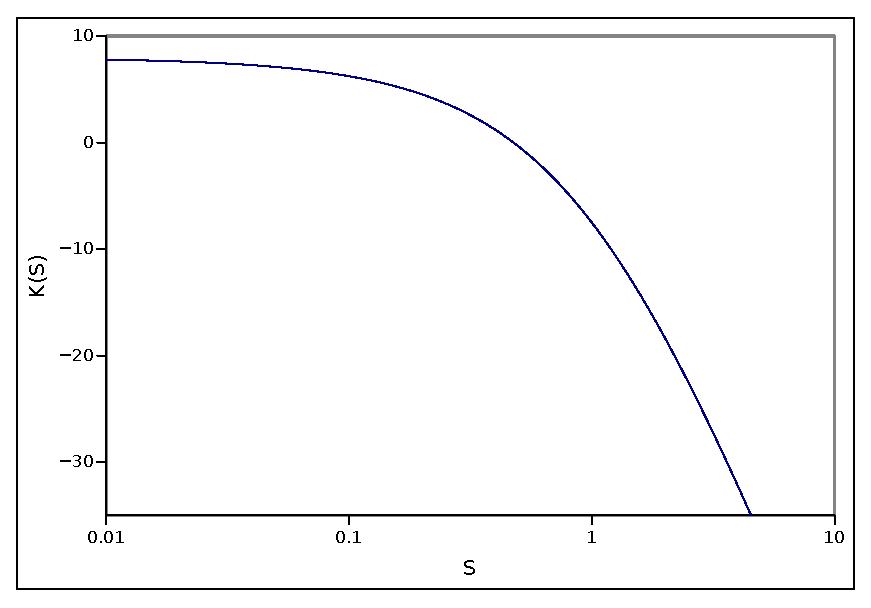
\includegraphics[scale=1]{charakterystyka_log}
\caption{Charakterystyka logarytmiczna}
\end{figure}
\end{document}